\documentclass[11pt,a4paper, parskip=half ]{report}
\usepackage[aux]{rerunfilecheck}
\usepackage{polyglossia}
\setmainlanguage{german}
\usepackage[utf8x]{inputenc}
%\usepackage{floatflt}
\usepackage{float}
\floatplacement{figure}{htbp}
\floatplacement{table}{htbp}
\pagestyle{empty}
\usepackage{multicol}
\usepackage{graphicx}
\usepackage{amssymb}
\usepackage{amsmath}
\usepackage{xparse}
\usepackage{braket}
\usepackage{units}
\usepackage[locale=DE,separate-uncertainty=true,per-mode=reciprocal,output-decimal-marker={,},]{siunitx}
\usepackage[section]{placeins}
\usepackage{pdflscape}
\usepackage{expl3}
\usepackage{bookmark}
\usepackage{sidecap}
%Komma als Dezimaltrenner in der mathe Umgebung, um in Umgebungen wie [0, 2] ein Leerzeichen nach dem Komma zu erhalten einfach eins setzen
\usepackage{icomma}
\textwidth16.5cm
\textheight26.5cm
\oddsidemargin0cm \evensidemargin-0.5cm \topmargin-1.5cm
\setlength{\parindent}{0pt}

\renewcommand{\labelenumi}{\alph{enumi})}
\newcommand{\Einheit}[1]{\ensuremath{\,\mathrm{#1}}}
\newcommand{\FracEinheit}[2]{\ensuremath{\,\frac{\mathrm{#1}}{\mathrm{#2}}}}
\newcommand{\difft}{\ensuremath{\,\frac{\mathrm{d}}{\mathrm{d}t}}\,}
\newcommand{\diffpr}{\ensuremath{\,\frac{\partial}{\partial r}}\,}
\newcommand{\diffptheta}{\ensuremath{\,\frac{\partial}{\partial \theta}}\,}
\newcommand{\diffpptheta}{\ensuremath{\,\frac{\partial^2}{\partial \theta^2}}\,}
\newcommand{\diffpphi}{\ensuremath{\,\frac{\partial}{\partial \phi}}\,}
\newcommand{\diffppphi}{\ensuremath{\,\frac{\partial^2}{\partial \phi^2}}\,}
\newcommand{\difftt}{\ensuremath{\,\frac{\mathrm{d}^2}{\mathrm{d}t^2}}\,}
\newcommand{\diffx}{\ensuremath{\,\frac{\mathrm{d}}{\mathrm{d}x}}\,}
\newcommand{\diffxx}{\ensuremath{\,\frac{\mathrm{d}^2}{\mathrm{d}x^2}}\,}
\newcommand{\vek}[2]{\ensuremath{\left( \begin{array}{c}#1\\#2\end{array} \right)}}
\newcommand{\vektor}[3]{\ensuremath{\left( \begin{array}{c}#1\\#2\\#3\end{array} \right)}}
\newcommand{\KleinerAbstand}{\\[5pt]}
\newcommand{\GrosserAbstand}{\\[12pt]}
\newcommand{\NaechsteSeite}{\begin{flushright}\textit{bitte wenden!}\end{flushright}\newpage}
\newcommand{\NaechstesBlatt}{\begin{flushright}\textit{weiter auf zweitem Blatt!}\end{flushright}\newpage}
\graphicspath{{../Bilder/}}
%\hyphenation{}


%%%%%%%%%%%%%%%%%%%%%%%%%%%%%%%%%%%%%
%% Deklarierung eigenere Operatoren%%
%%%%%%%%%%%%%%%%%%%%%%%%%%%%%%%%%%%%%
\DeclareMathOperator{\Div}{div}
\DeclareMathOperator{\Rot}{rot}
%%%%%%%%%%%%%%%%%%%%%%%%%%%%%%%%%%%%%


\begin{document}


\includegraphics[width=\textwidth]{logo_tu_fp.png}
%\GrosserAbstand
\begin{center}
\Large{\textbf{4. \"Ubungsblatt zum Vorkurs Physik}}
\GrosserAbstand
\normalsize
Wintersemester 2020/21 \hfill Prof. Dr. Carsten Westphal\\
\textbf{Für den 22.10.2020} \hfill Prof. Dr. Jan Kierfeld \\
\end{center}

%
%
% * * * * * * * * * * * * * * * * * * * * *
%  AUFGABE 1
% * * * * * * * * * * * * * * * * * * * * *
%
%

\section*{Aufgabe 1: Erstes Mal Taylor-Entwicklung}
  Gegeben ist $f(x) = \sqrt[3]{2x + 2}, \quad x \geq -1$.
  \begin{enumerate}
    \item Bestimmen Sie die ersten zwei Ableitungen der Funktion $f$.
    \item Stellen Sie das Taylorpolynom $2.$ Grades von $f$ mit Entwicklungspunkt $x_0 = 3$ auf.
  \end{enumerate}

  \section*{Aufgabe 2: Von Taylor-\textit{Entwicklung} zu Taylor\textit{reihe}}
  Berechnen Sie alle Ableitungen $f^{(n)}$ mit $n = 0, 1, 2, ...$ der Funktion $f$ und geben Sie damit die Taylorreihe für $f$ mit Entwicklungspunkt $x_0 = 0$ an,  
  \begin{enumerate}
    \item $f(x) = \sin(3x), \,\, x \in \mathbb{R}$, 
    \item $f(x) = \sqrt{1+x}, \,\,|x| \leq 1$.
  \end{enumerate}

  \section*{Aufgabe 3: Taylor-Entwicklung die Zweite}
  Bestimmen Sie das Taylorpolynom dritten Grades der Funktion $f(x) = e^{\sin(x)}$ im Entwicklungspunkt $x_0 = 0$.   

  \section*{Aufgabe 4:  Taylor-Entwicklung die Letzte*}
  Bestimmen Sie das Taylorpolynom dritten Grades der Funktion \begin{enumerate}
    \item $f(x) = \sin(x)$ mit $x_0 = 0$,
    \item $f(x) = x \ln(x)$ mit $x_0 = 1$. 
  \end{enumerate}

\vfill
\begin{flushright}\textit{Seite 1 von 2}\end{flushright}\newpage


\section*{Aufgabe 5: Kurvendiskussion}
\begin{enumerate}
  \item Bestimmen Sie die Extrempunkte der Funktion f mit $f(x) = e^{2x} + e^{-x}$.
  \item Bestimmen Sie den Wendepunkt der Funktion f mit $f(x) = (x-1)\cdot e^x$.
\end{enumerate}

\section*{Aufgabe 6: Und weil's so schön war Kurvendiskussion}
\begin{enumerate}
  \item Die Funktion f  hat das nebenstehende Schaubild und die	Funktionsgleichung $f(x) = a\cdot e^x + b$ mit $(a,b \in \mathbb{R})$. Bestimmen Sie die Werte von a und b. Tipp: Betrachten Sie den Verlauf der Funktion.
  \begin{figure}
    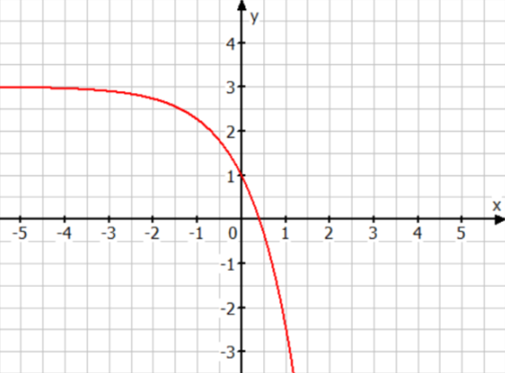
\includegraphics{media/Bild1.png}
  \end{figure}
  \item Gegeben sind die Funktionen f und g mit $f(x) = \frac{1}{1-x}+3$ und $g(x)=-\frac{1}{1+x}$.	Geben Sie die waagrechte Asymptote der Funktion f an und bestimmen Sie die Stelle, an der f und g  die gleiche Steigung haben.
\end{enumerate}


\vfill
\begin{flushright}\textit{Seite 2 von 2}\end{flushright}%\newpage

\end{document}
